\subsection{A full-run wall-time record}\label{app:latest-round-clock}

Logged round durations span the admission period
(\cref{fig:fw-latest-round-clock}); these operating clocks are separate from
the admission counts in \cref{tab:admission-ledger}.
Pricing a game-day proposal still requires \mbox{the full attempt} ledger (\cref{sub:price-run}).

% Graphic left, caption right (as Figure 40): a column-width graphic alone left the other column empty under the full-width figures.
\begin{figure*}[!t]
  \setlength{\abovecaptionskip}{4pt}
  \begin{minipage}[t]{\dimexpr.5\textwidth-.5\columnsep\relax}
  \vspace{0pt}
  \centering
  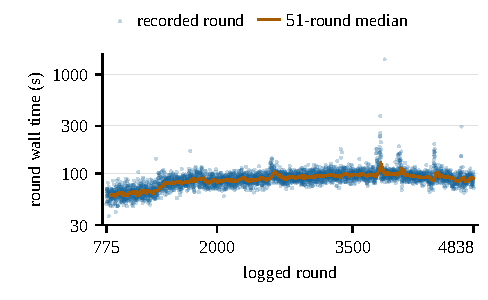
\includegraphics[width=\linewidth]{figures/fig_fw_latest_round_clock.pdf}
  \end{minipage}\hfill
  \begin{minipage}[t]{\dimexpr.5\textwidth-.5\columnsep\relax}
  \vspace{0pt}
  \caption{\textbf{Recorded round durations vary across the full admission period.}
  All \num{4064} retained wall-time records in rounds 775--4838, captured at
  04:58 UTC on 4 November 2026. Each point is a logged round's wall seconds;
  the line is the trailing 51-round median, starting with the 51st record.
  The vertical axis is logarithmic; no raw duration is filtered.
  These clocks include timed in-round work and waits, not inter-round gaps
  or single-proposal latency. Scope: \cref{sec:method-status}.}
  \label{fig:fw-latest-round-clock}
  \end{minipage}
\end{figure*}
